%%\documentclass[tikz]{standalone}
%
%%% Language and font encodings
%\usepackage[english]{babel}
%\usepackage[utf8x]{inputenc}
%\usepackage[T1]{fontenc}
%


% Define parallelepiped shape:
\makeatletter
\pgfkeys{/pgf/.cd,
  parallelepiped offset x/.initial=2mm,
  parallelepiped offset y/.initial=2mm
}
\pgfdeclareshape{parallelepiped}
{
  \inheritsavedanchors[from=rectangle] % this is nearly a rectangle
  \inheritanchorborder[from=rectangle]
  \inheritanchor[from=rectangle]{north}
  \inheritanchor[from=rectangle]{north west}
  \inheritanchor[from=rectangle]{north east}
  \inheritanchor[from=rectangle]{center}
  \inheritanchor[from=rectangle]{west}
  \inheritanchor[from=rectangle]{east}
  \inheritanchor[from=rectangle]{mid}
  \inheritanchor[from=rectangle]{mid west}
  \inheritanchor[from=rectangle]{mid east}
  \inheritanchor[from=rectangle]{base}
  \inheritanchor[from=rectangle]{base west}
  \inheritanchor[from=rectangle]{base east}
  \inheritanchor[from=rectangle]{south}
  \inheritanchor[from=rectangle]{south west}
  \inheritanchor[from=rectangle]{south east}
  \backgroundpath{
    % store lower right in xa/ya and upper right in xb/yb
    \southwest \pgf@xa=\pgf@x \pgf@ya=\pgf@y
    \northeast \pgf@xb=\pgf@x \pgf@yb=\pgf@y
    \pgfmathsetlength\pgfutil@tempdima{\pgfkeysvalueof{/pgf/parallelepiped
      offset x}}
    \pgfmathsetlength\pgfutil@tempdimb{\pgfkeysvalueof{/pgf/parallelepiped
      offset y}}
    \def\ppd@offset{\pgfpoint{\pgfutil@tempdima}{\pgfutil@tempdimb}}
    \pgfpathmoveto{\pgfqpoint{\pgf@xa}{\pgf@ya}}
    \pgfpathlineto{\pgfqpoint{\pgf@xb}{\pgf@ya}}
    \pgfpathlineto{\pgfqpoint{\pgf@xb}{\pgf@yb}}
    \pgfpathlineto{\pgfqpoint{\pgf@xa}{\pgf@yb}}
    \pgfpathclose
    \pgfpathmoveto{\pgfqpoint{\pgf@xb}{\pgf@ya}}
    \pgfpathlineto{\pgfpointadd{\pgfpoint{\pgf@xb}{\pgf@ya}}{\ppd@offset}}
    \pgfpathlineto{\pgfpointadd{\pgfpoint{\pgf@xb}{\pgf@yb}}{\ppd@offset}}
    \pgfpathlineto{\pgfpointadd{\pgfpoint{\pgf@xa}{\pgf@yb}}{\ppd@offset}}
    \pgfpathlineto{\pgfqpoint{\pgf@xa}{\pgf@yb}}
    \pgfpathmoveto{\pgfqpoint{\pgf@xb}{\pgf@yb}}
    \pgfpathlineto{\pgfpointadd{\pgfpoint{\pgf@xb}{\pgf@yb}}{\ppd@offset}}
  }
}
\makeatother

\tikzset{
  % Dark blue blocks
  block/.style={
    parallelepiped,fill=white, draw,
    minimum width=0.8cm,
    minimum height=2.4cm,
    parallelepiped offset x=0.5cm,
    parallelepiped offset y=0.5cm,
    path picture={
      \draw[top color=darkblue,bottom color=darkblue]
        (path picture bounding box.south west) rectangle
        (path picture bounding box.north east);
    },
    text=white,
  },
  % Orange-ish blocks
  conv/.style={
    parallelepiped,fill=white, draw,
    minimum width=0.8cm,
    minimum height=2.4cm,
    parallelepiped offset x=0.5cm,
    parallelepiped offset y=0.5cm,
    path picture={
      \draw[top color=salmon,bottom color=salmon]
        (path picture bounding box.south west) rectangle
        (path picture bounding box.north east);
    },
    text=white,
  },
  % Taller Light blue blocks:
  plate/.style={
    parallelepiped,fill=white, draw,
    minimum width=0.1cm,
    minimum height=7.4cm,
    parallelepiped offset x=0.5cm,
    parallelepiped offset y=0.5cm,
    path picture={
      \draw[top color=lightblue,bottom color=lightblue]
        (path picture bounding box.south west) rectangle
        (path picture bounding box.north east);
    },
    text=white,
  },
  % Arrows between blocks:
  link/.style={
    color=lightblue,
    line width=2mm,
  },
}


\begin{tikzpicture}
  % The order of blocks matters since some are partially hidden behind subsequent blocks.
  \node[conv](conv1){\rotatebox{90}{Conv}};
  \node[plate,right=0.2cm of conv1](plate1){};
  % yshift to align the bottom of that blocks with the previous taller block.
  \node[block,right=0.2cm of plate1,yshift=-2.5cm](resblock1){\rotatebox{90}{ResBlock}};
  \node[block,above=0.1cm of resblock1](resblock2){\rotatebox{90}{ResBlock}};
  \node[block,above=0.1cm of resblock2](resblock3){\rotatebox{90}{ResBlock}};
  \node[block,right=0.2cm of resblock1](x1){\rotatebox{90}{(X4)}};
  \node[block,above=0.1cm of x1](x2){\rotatebox{90}{(X3)}};
  \node[block,above=0.1cm of x2](x3){\rotatebox{90}{(X2)}};
  \node[plate,right=0.2cm of x2](plate2){};
  \node[block,right=0.6cm of x2](resblock4){\rotatebox{90}{ResBlock4}};
  \node[block,right=2cm of resblock4](resblock5){\rotatebox{90}{ResBlock5}};
  \node[conv,right=0.2cm of resblock5](conv2){\rotatebox{90}{Conv}};
  \draw [-,link] ([xshift=0.2cm,yshift=0.2cm]resblock4.east) -- ([yshift=0.2cm]resblock5.west);
  \draw [-triangle 60,link] ([xshift=0.2cm,yshift=0.2cm]conv2.east) -- ([xshift=1.5cm,yshift=0.2cm]conv2.east);
\end{tikzpicture}


\section{Artificial Neural Networks}\label{sec:neural-networks}
\localtableofcontents
Artificial Neural Network algorithms for SR are all based on a Convolutional Neural Network (CNN) architecture. 
%
We first briefly review ANNs in general and CNNs in particular and then explore the recent advances in Deep Learning (DL) for SR.
%
\subsection{Basics}
\begin{figure*}
    % MLP
    \centering
    \tikzstyle{inputNode}=[draw,fill=sail,circle,minimum size=10pt,inner sep=2pt]
    \tikzstyle{hiddenNode}=[draw,fill=snowymint,circle,minimum size=10pt,inner sep=2pt]
    \tikzstyle{outputNode}=[draw,fill=plum,circle,minimum size=10pt,inner sep=2pt]
    \tikzstyle{stateTransition}=[-stealth, thick]
    \begin{subfigure}[b]{0.49\textwidth}
        \centering
        \begin{tikzpicture}
            \node[draw,fill=plum, circle,minimum size=25pt,inner sep=0pt] (x) at (0,0) {$\Sigma$ $\sigma$};
            \draw[dashed] (0,-0.43) -- (0,0.43);

            \node[inputNode] (x0) at (-2, 1.5) {$ x_1$};
            \node[inputNode] (x1) at (-2, 0.75) {$ x_2$};
            \node[inputNode] (x2) at (-2, 0) {$ x_3$};
            \node[inputNode] (x3) at (-2, -0.75) {$ x_4$};
            \node[inputNode] (xn) at (-2, -1.95) {$ x_n$};

            \draw[stateTransition] (x0) to[out=0,in=120] node [midway, sloped, above] {$w_1$} (x);
            \draw[stateTransition] (x1) to[out=0,in=150] node [midway, sloped, above] {$w_2$} (x);
            \draw[stateTransition] (x2) to[out=0,in=180] node [midway, sloped, above] {$w_3$} (x);
            \draw[stateTransition] (x3) to[out=0,in=210] node [midway, sloped, above] {$w_4$} (x);
            \draw[stateTransition] (xn) to[out=0,in=240] node [midway, sloped, above] {$w_n$} (x);
            \draw[stateTransition] (x) -- (4,0) node [midway,above] {$z(\mathbf{x}) = \sigma\left(\sum\limits_{i=1}^{n}{w_ix_i} +  b\right)$};
            \node (dots) at (-2, -1.25) {$\vdots$};
        \end{tikzpicture}
        \caption{Single Artificial Neuron function.}\label{fig:singleann}
    \end{subfigure}
    \begin{subfigure}[b]{0.49\textwidth}
        \centering
        \begin{tikzpicture}

            \node[inputNode, thick] (i1) at (6, 0.75) {$x_1$};
            \node[inputNode, thick] (i2) at (6, 0) {$x_2$};
            \node[] (i4) at (6, -0.75) {$\LARGE \vdots$};
            \node[inputNode, thick] (i3) at (6, -1.5) {$x_n$};

            \node[hiddenNode, thick] (h1) at (8, 1.5) {$z_1$};
            \node[hiddenNode, thick] (h2) at (8, 0.75) {$z_2$};
            \node[hiddenNode, thick] (h3) at (8, 0) {$z_3$};
            \node[] (h4) at (8, -0.75) {$\LARGE \vdots$};
            \node[]  at (8, -1.5) {$\LARGE \vdots$};
            \node[hiddenNode, thick] (h5) at (8, -2.25) {$z_m$};

            \node[outputNode, thick] (o2) at (10, 0) {$\Sigma$ $\sigma$};
            \draw[dashed] (10,-0.43) -- (10,0.43);

            \draw[stateTransition] (i1) -- (h1);
            \draw[stateTransition] (i1) -- (h2);
            \draw[stateTransition] (i1) -- (h3);
            \draw[stateTransition] (i1) -- (h5);
            \draw[stateTransition] (i2) -- (h1);
            \draw[stateTransition] (i2) -- (h2);
            \draw[stateTransition] (i2) -- (h3);
            \draw[stateTransition] (i2) -- (h5);
            \draw[stateTransition] (i3) -- (h1);
            \draw[stateTransition] (i3) -- (h2);
            \draw[stateTransition] (i3) -- (h3);
            \draw[stateTransition] (i3) -- (h5);

            \draw[stateTransition] (h1) -- (o2);
            \draw[stateTransition] (h2) -- (o2);
            \draw[stateTransition] (h3) -- (o2);
            \draw[stateTransition] (h5) -- (o2);

            \node[above=of i1, align=center] (l1) {\footnotesize $n$ Neuron \\ \footnotesize Input \\ \footnotesize layer};
            \node[right=1.3em of l1, align=center] (l2) {\footnotesize $m$ Neuron \\ \footnotesize Hidden \\ \footnotesize layer};
            \node[right=2.3em of l2, align=center] (l3) {\footnotesize Output \\ \footnotesize layer};

            \draw[stateTransition] (o2) -- node[midway,above] {$y(\mathbf{x}) = \sigma'\left(\sum\limits_{j=1}^{m}{w'_jz_j} + b'\right)$} (13, 0);
        \end{tikzpicture}
        \caption{Multi-layer ANN.}\label{fig:multiann}
    \end{subfigure}
    \caption{Artificial Neural Network representation.}\label{fig:ann}
\end{figure*}

An Artificial Neural Network (ANN or NN) is a function specified by compositions of elementary functions called \textit{artificial neurons}\anote{ann} (or simply neurons).
%
Neurons consist of a set of inputs \(x_1, x_2, \dots, x_n\), an aggregation (typically summation), and an activation function \(\sigma\), which acts as a thresholding mechanism. 
%
For example, the simplest function that qualifies as a neuron is a linear function:
\begin{equation}
    y = x_1 + x_2 = \sum_i x_i
\end{equation}
where the the activation function is the trivial one i.e., the identity.
%
Common non-trivial, i.e., non-linear, activation functions are the sigmoid function
\begin{equation}
    S(x)={\frac {1}{1+e^{-x}}}={\frac {e^{x}}{e^{x}+1}}
\end{equation}
or the hyperbolic tangent function 
\begin{equation}
    \tanh x={\frac {\sinh x}{\cosh x}}={\frac {e^{x}-e^{-x}}{e^{x}+e^{-x}}}={\frac {e^{2x}-1}{e^{2x}+1}}
\end{equation}
or the piece-wise defined \textit{rectified linear unit} (\(\operatorname{ReLU}\))
\begin{align}
\operatorname{ReLU}(x) &=\begin{cases}x&{\text{if }}x>0,\\0&{\text{otherwise}}\end{cases} \\ 
    &= \max(0, x)
\end{align}
%
Minsky \etal\cite{minsky2017perceptrons} famously proved that neurons that don't include a non-linear activation function have very little approximation power (i.e., they're unable to approximate functions as simple as even \(\operatorname{XOR}\)\anote{xor}.) and those that do are universal approximators (i.e., given enough layers and neurons they're able to approximate functions of arbitrary complexity).
%
Note that this linear function passes through the origin \((0,0,0)\) since it has no constant term; in the parlance of machine learning the neuron is missing a bias term\anote{bias} \(b\):
\begin{equation}
    y = x_1 + x_2 + b
    \label{eqn:linearregr}
\end{equation}
%
ANNs are then assemblies of neurons grouped into \textit{layers} with the layers composed by applying neurons to weighted outputs from immediately preceding layers.
%
Those layers that are not input or output layers are denoted \textit{hidden} layers.
%
These \textit{networks} can be represented as directed graphs where vertices represent neurons and edges represent composition weights (see figure~\ref{fig:ann}).
%
For example the ANN specified in figure~\ref{fig:ann} represents the function 
\begin{align}
    y &= \sigma' \left( \sum_j w'_j z_j + b' \right) \\
      &=  \sigma' \left( \sum_{j=1}^m w'_j \sigma\left(\sum_{i=1}^n w_i x_i + b_j\right) + b' \right)
\end{align}



\begin{figure*}
    \centering
    \begin{subfigure}[b]{0.33\textwidth}
        \centering
        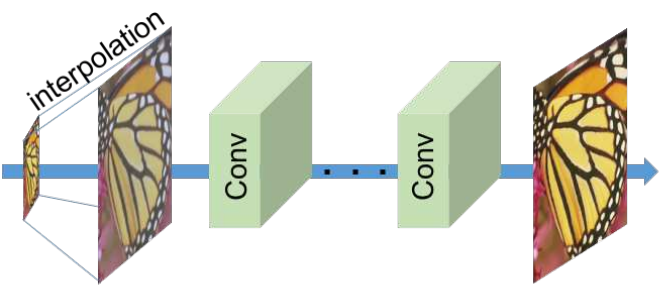
\includegraphics[width=0.95\textwidth]{figures/neural_networks/predefined_upsample.png}
        \caption{Predefined up-sampling.}\label{fig:predefups}
    \end{subfigure}
    \begin{subfigure}[b]{0.66\textwidth}
        \centering
        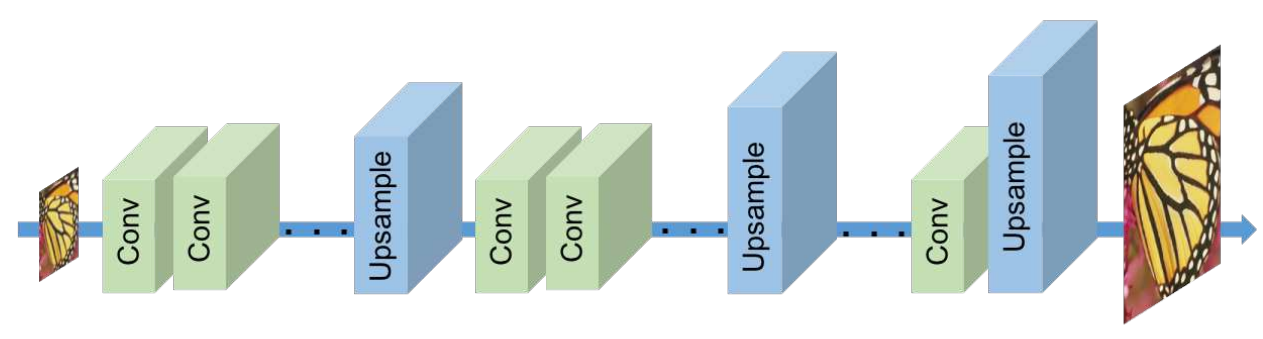
\includegraphics[width=0.95\textwidth]{figures/neural_networks/progressive_upsample.png}
        \caption{Progressive up-sampling.}\label{fig:profups}
    \end{subfigure}

    \begin{subfigure}[b]{0.33\textwidth}
        \centering
        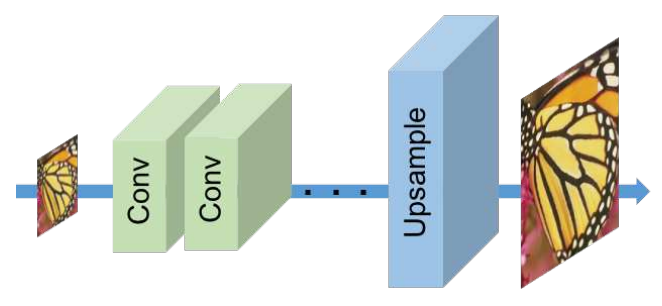
\includegraphics[width=0.95\textwidth]{figures/neural_networks/single_upsample.png}
        \caption{Single up-sampling.}\label{fig:singups}
    \end{subfigure}
    \begin{subfigure}[b]{0.66\textwidth}
        \centering
        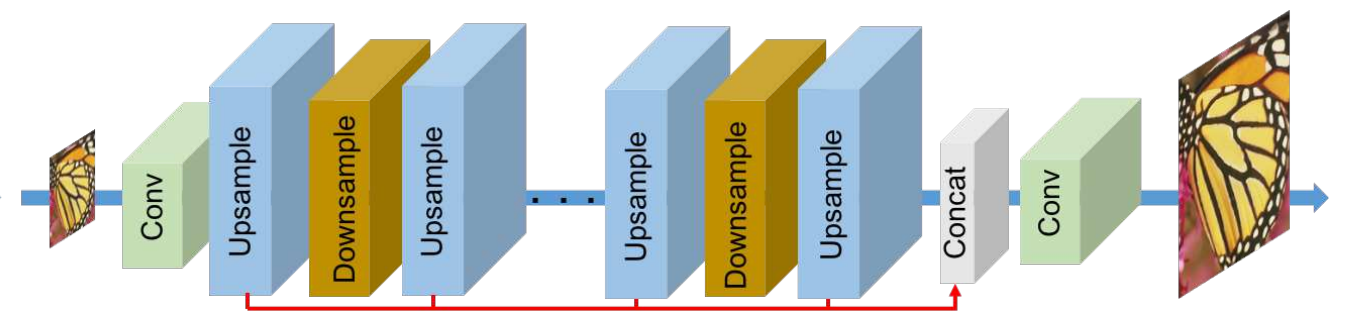
\includegraphics[width=0.95\textwidth]{figures/neural_networks/iterative_upsample.png}
        \caption{Iterative up-down-up-sampling.}\label{fig:iterups}
    \end{subfigure}
    \caption{Comparison of Deep SR network architectures \cite{haris2018deep}}\label{fig:comparedeepsr}
\end{figure*}